\documentclass{beamer}
\usepackage{amsmath}
\usepackage[utf8]{inputenc}
\usepackage{hyperref}
\usepackage{multicol}
\usepackage{hyperref}
\usepackage{xcolor}

\inputencoding{utf8}

\mode<presentation> {
    \usetheme{Madrid}
}

\usepackage{graphicx}
\usepackage{booktabs}

\title[Relaciones]{Relaciones}
\author{Ernesto Rodriguez}
\institute{
    Universidad del Itsmo \\
    \medskip \textit{erodriguez@unis.edu.gt}
}

\date[\today]{}

\begin{document}

\begin{frame}
    \maketitle
\end{frame}

\begin{frame}
\frametitle{Tipos inductivos en Elm}
\begin{itemize}
    \item{Elm permite declarar conjuntos de valores (conocidos
    como {\bf tipos}) mediante la palabra reservada {\bf type}.
    \begin{itemize}
        \item{$\mathbf{type}\ \mathtt{Booleano=T\ |\ F}$}
        \item{$\mathbf{type}\ \mathtt{Natural=Succ\ Natural\ |\ Cero}$}
    \end{itemize}
    }
    \item{Los tipos se dividen en {\bf casos}, cada caso se separa
    mediante `` $\vert$ ''.}
    \item{Un tipo puede tener una cantidad arbitraria de casos distintos.}
    \item{Los casos pueden ser {\bf recursivos}, similar a nuestra definici\'on
    original de {\bf Naturales Unarios}}
\end{itemize}
\end{frame}

\begin{frame}
\frametitle{Utilizaci\'on de Tipos}
\begin{itemize}
    \item{Se pueden definir funci\'ones para valores de nuestros tipos
    nuevos mediante {\bf analisis de casos}, coloquialmente conocido como
    {\bf pattern matching}.}
    \item{Elm (a diferencia de SML, Haskell, etc.) requiere que los casos
    sean {\bf exahustivos}, es decir que se abarquen todos los casos.
    \begin{itemize}
        \item{Ayuda a mejorar la robustez de nuestro codigo}
        \item{Puede ser dificil agregar casos nuevos a tipos existentes}
    \end{itemize}
    }
    \item{Elm tampoco permite {\bf casos reduntantes}, ya que pueden llevar
    a {\bf inconsistencias}.}
\end{itemize}

\begin{center}
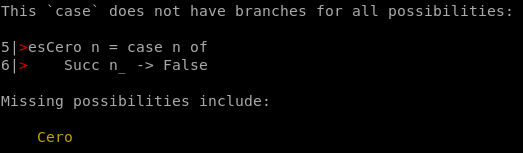
\includegraphics[width=5cm]{./missing.png}
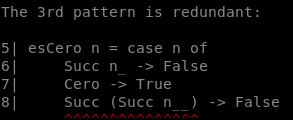
\includegraphics[width=5cm]{./redundant.png}
\end{center}

\end{frame}

\begin{frame}
\frametitle{Ejemplo: Dias de la Semana}
\begin{itemize}
    \item{Definici\'on del tipo: \\
    $>\ \mathbf{type}\ \mathtt{dia\ =\ Lun\ |\ Mar\ |\ Mie\ |\ 
    Jue\ |\ Vie\ |\ Sab\ |\ Dom}$}
    \item{Funci\'on para reconocer dias de trabajo:\vspace{0.5cm}
    $
        \begin{array}{ll}
            \mathtt{diaDeTrabajo}\ dia=&\mathbf{case}\ dia\ \mathbf{of} \\
            & \ \ \mathtt{Sab} \rightarrow \mathtt{False} \\
            & \ \ \mathtt{Dom} \rightarrow \mathtt{False} \\
            & \ \ \_ \rightarrow \mathtt{True}
        \end{array}
    $}
    \item{Es possible utilizar la funci\'on:\\
    $>\mathtt{diaDeTrabajo}\ \mathtt{Dom}$\\
    $\mathtt{False}$}
\end{itemize}
\end{frame}

\begin{frame}
\frametitle{Ejemplo: Numeros Naturales Unarios}
Ver la carpeta de de ejemplos (``../ejemplos'')
\end{frame}

\begin{frame}
    \frametitle{Abstraccion: Representando objetos como tipos}
    \begin{itemize}
        \item{Se describiran tres figuras geometricas diferentes:
        \begin{center}
            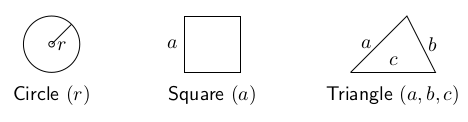
\includegraphics[width=8cm]{./figuras.png}
        \end{center}
        {\bf Matematicamente: $\mathbb{R^+}\uplus\mathbb{R^+}\uplus(\mathbb{R^+}\times\mathbb{R^+}\times\mathbb{R^+})$}
        }
        \item{En Elm, el conjunto $\mathbb{R}$ se aproximara mediante el tipo
        $\mathtt{Float}$}
        \item{Esto permite definir las figuras por casos:}
    \end{itemize}

\end{frame}

\begin{frame}
    \frametitle{Abstraccion: Representando objetos como tipos}
    \begin{itemize}
        \item{Se describiran tres figuras geometricas diferentes:
        \begin{center}
            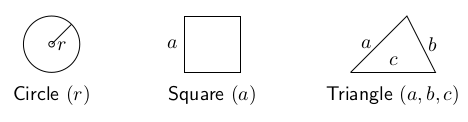
\includegraphics[width=8cm]{./figuras.png}
        \end{center}
        {\bf Matematicamente: $\mathbb{R^+}\uplus\mathbb{R^+}\uplus(\mathbb{R^+}\times\mathbb{R^+}\times\mathbb{R^+})$}
        }
        \item{En Elm, el conjunto $\mathbb{R}$ se aproximara mediante el tipo
        $\mathtt{Float}$}
        \item{Esto permite definir las figuras por casos:\\
        $
        \begin{array}{ll}
            \mathbf{type}\ \mathtt{Figura=} & \mathtt{Circulo\ Float}\\
            & |\ \mathtt{Cuadrado\ Float} \\
            & |\ \mathtt{Triangulo\ (Float,Float,Float)}
        \end{array}    
        $}
    \end{itemize}

\end{frame}

\begin{frame}
\frametitle{Abstracci\'on: Area de Figuras}
Ver la carpeta de de ejemplos (``../ejemplos'')
\end{frame}

\end{document}